\documentclass{article}
\linespread{1.3}
\usepackage[margin=50pt]{geometry}
\usepackage{amsmath, amsthm, amssymb, amsthm, tikz, fancyhdr, graphicx}
\pagestyle{fancy}
\renewcommand{\headrulewidth}{0pt}
\newcommand{\changefont}{\fontsize{15}{15}\selectfont}

\fancypagestyle{firstpageheader}
{
  \fancyhead[R]{\changefont Michael Huang \\ CFRM 420 \\ Homework 6}
}

\begin{document}

\thispagestyle{firstpageheader}

\section*{1.}
{\Large 

% \begin{verbatim}
%   Text enclosed inside \texttt{verbatim}
%   environment 
%   is printed directly 
%   and all \LaTeX{} commands are ignored.
% \end{verbatim}

% \framebox[1.1\width]{\textbf{answer}}

\subsection*{(a)}

We implement this in R. One value that is generated is \\
\framebox[1.1\width]{\textbf{Estimate: 0.6739545}}

\subsection*{(b)}

We implement this in R. The bootstrap statistics are \\
\framebox[1.1\width]{\textbf{Estimate: 0.6687307}} \\
\framebox[1.1\width]{\textbf{Bias: 6.870455e-05}} \\
\framebox[1.1\width]{\textbf{Std. error: 0.01524621}}

\subsection*{(c)}

We plot in R, and the distribution does seem to be approximately normal, with slightly lower tails than the normal distribution line:
\begin{figure}[h!]
  \centering
  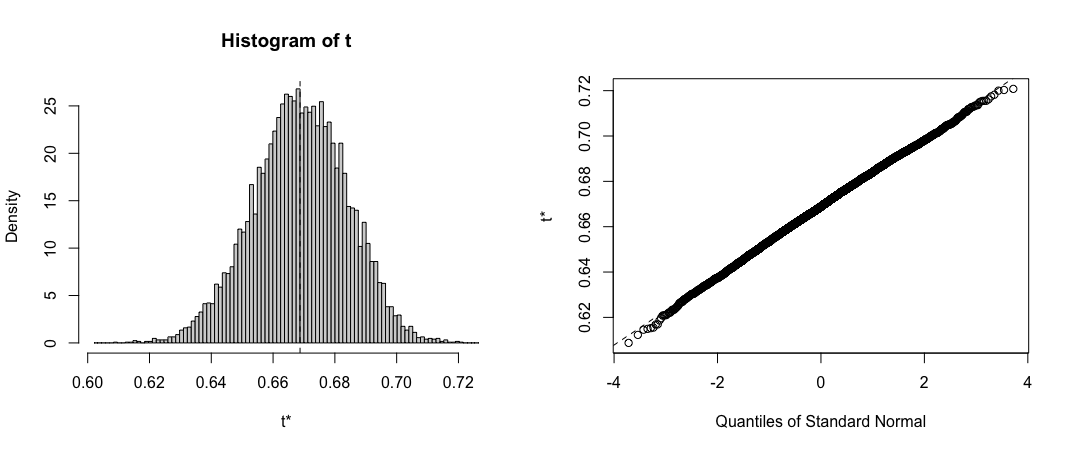
\includegraphics[width=500pt]{hw6_1c.png}
\end{figure}

\subsection*{(d)}

We implement this in R, and get the following values: \\ 
\framebox[1.1\width]{\textbf{Normal 95\% CI: ( 0.6388,  0.6985 )}} \\ 
\framebox[1.1\width]{\textbf{Percentile 95\% CI: ( 0.6379,  0.6976 )}}

\subsection*{(e)}

We can calculate the approximate 95\% confidence interval for $\hat{\rho}$ as given, with the fact that $n = 3626$ and $\hat{\rho} = 0.6687307$ as we find using R: \\
$(\hat{\rho} - 1.96 \frac{1 - \hat{\rho}^2}{\sqrt{n}}, \hat{\rho} + 1.96 \frac{1 - \hat{\rho}^2}{\sqrt{n}})$ \\
= $(0.6687307 - 1.96 \cdot \frac{1 - 0.6687307^2}{\sqrt{3626}}, 0.6687307 + 1.96 \cdot \frac{1 - 0.6687307^2}{\sqrt{3626}})$ \\
= $(0.6687307 - 1.96 \cdot \frac{1 - 0.44720074912}{\sqrt{3626}}, 0.6687307 + 1.96 \cdot \frac{1 - 0.44720074912}{\sqrt{3626}})$ \\
= $(0.6687307 - 1.96 \cdot \frac{0.55279925088}{\sqrt{3626}}, 0.6687307 + 1.96 \cdot \frac{0.55279925088}{\sqrt{3626}})$ \\
= $(0.6687307 - 1.96 \cdot 0.00918022965, 0.6687307 + 1.96 \cdot 0.00918022965)$ \\
= $(0.6687307 - 0.01799325011, 0.6687307 + 0.01799325011)$ \\
= $(0.65073744989, 0.68672395011)$ \\
This approximate 95\% confidence interval seems to be relatively close, but much smaller and thus more refined than both of the confidence intervals that we previously found. In this case, it seems that this calculated 95\% confidence interval is the most refined and therefore the most appropriate in this situation.
\newpage

}

\section*{2.}
{\Large

\subsection*{(a)}

We calculate and plot this using R, and it seems that the distribution is a bit skewed and not normal:
\begin{figure}[h!]
  \centering
  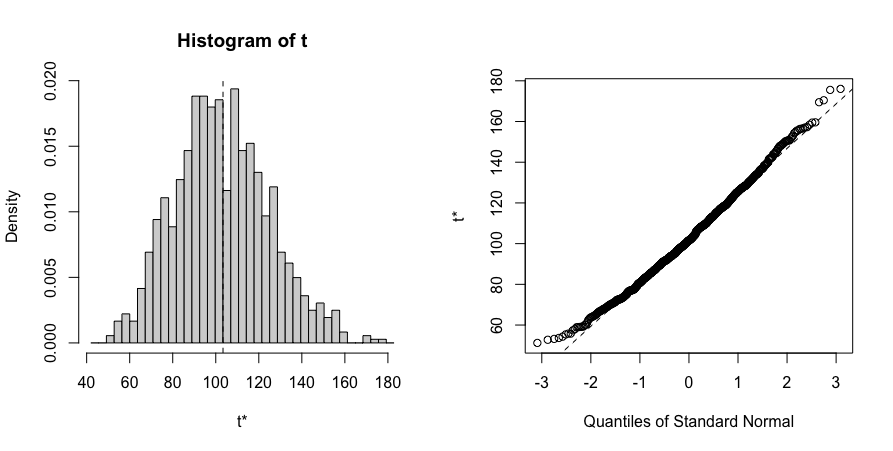
\includegraphics[width=500pt]{hw6_2a.png}
\end{figure}

\subsection*{(b)}

We implement this in R, and get the following results: \\
\framebox[1.1\width]{\textbf{Normal 90\% CI: ( 67.7, 139.6 )}} \\
\framebox[1.1\width]{\textbf{Percentile 90\% CI: ( 69.4, 141.8 )}} \\
\framebox[1.1\width]{\textbf{BCa 90\% CI: ( 74.5, 152.3 )}}

\subsection*{(c)}

See R file for specific implementation. I achieved the following results: \\
Normal: 0.869 \\ 
Percentile: 0.87 \\
BCa: 0.876 \\
where we attempt to measure how each method performed by measuring $\mathbb{P}(A \leq \beta \leq B)$ for the lower and upper limits of the confidence interval. From these results, the performance seems to be relatively close, but BCa seems to perform the best, with Percentile next best, and Normal following, which was extremely close in terms of performance.

}

\end{document}